\documentclass{article}
\usepackage[utf8]{inputenc}
\usepackage{amsmath}
\usepackage[letterpaper, portrait, margin=1in]{geometry}
\usepackage{graphicx}
\graphicspath{{images/}}

\begin{document}
\title{Projeto Demonstrativo 2 - Calibração de câmeras}
\date{23-04-2016}
\author{Samuel Venzi Lima Monteiro de Oliveira\\14/0162241\\samuel.venzi@me.com}

	\maketitle
	\pagenumbering{arabic}

	\section{Objetivos}
		\paragraph{}
		O objetivo deste processo é realizar um estudo sobre câmera e sua calibração. A partir desse estudo, desenvolver um método para calculo de dimensões de objetos dada a distância entre este e a câmera.
	\section{Introdução}
		\paragraph{}
		O uso de câmeras no âmbito da visão computacional é uma competência essencial devido às inúmeras aplicações práticas existentes. Tais aplicações vão desde câmeras de vigilância até carros autônomos, portanto é necessário saber sobre o funcionamento de câmeras e entender seus detalhes para que seja bem aplicada. Os principais pontos abordados neste estudo são a calibração de câmeras e, a partir disso, a avaliação do tamanho de objetos no frame da imagem capturada.
		\paragraph{}
		A estrutura básica das câmeras atuais segue a estrutura consagrada pelos primeiros estudos feitos sobre capturas de imagens. O que essa estrutura permite é a entrada de luz por um orifício ou conjunto de lentes e sua projeção em um filme ou sensor que captura a imagem. As câmeras modernas utilizam lentes e sensores, e é importante entender como essas duas partes influenciam na maneira que deve se lidar com a manipulação de imagens dessas câmeras.
		\paragraph{}
		Com a introdução de lentes nas câmeras, foi possível a captura de imagens de muito melhor qualidade pois elas permitiam maior entrada de luz sem o desfoque da imagem, o que acontecia com o aumento do oríficio. Porém, a depender da qualidade de fabricação da lente, com elas ocorre o fenômeno da distorção que pode ser um grande problema para certas aplicações. No caso do uso de sensores, certas caracteríscas são importantes serem conhecidas, como seu tamanho e o tamanho de seus píxels.
		\paragraph{}
		A calibração da câmera tem como função anular certas distorções da imagem que possam ocorrer por sua parte física. Portanto, alinhando hardware e software pode-se ter a representação mais fiel possível e a partir dessa representação retirar informações de interesse.
		\begin{center}
			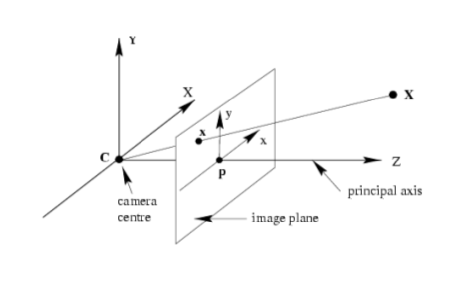
\includegraphics[scale=0.4]{CalibrationVariables}\\
			Figura 2.1
		\end{center}
		\paragraph{}
		Na figura 2.1 pode-se verificar algumas das variáveis de calibração. O sistema de referência é o plano da imagem, chamado também de frame e as coordenadas dos pixels no frame são dados por um par ordenado (x,y). 
		\paragraph{}
		A partir de estudos, são extraídas informções sobre a câmera, como seus parâmetros intrínsecos e extrínsicos. Onde os parâmetros intrínsecos caracterizam propriedades óticas, geométricas e digitais da câmera, além de sua distorção.
	\section{Materiais e Metodologia}
		\subsection{Materiais}
			\begin{itemize}
			\item Computador com ambiente Linux (Ubuntu)
			\item Câmera própria do computador
			\item OpenCV
			\item Bola com 6cm de diâmetro
			\end{itemize}
		\subsection{Metodologia}
			\paragraph{}
			Antes de mexer com a câmera em si, foi criada uma aplicação que captura o clique do mouse em dois pontos arbitrários da janela, desenha um linha e calcula a distância em pixels entre eles. O programa primeiramente cria uma imagem genérica, foi escolhida uma completamente preta, e com o uso de funções do OpenCV, captura e desenha uma linha ente dois pontos. Após isso ele calcula a distância Euclidiana Bidimensional.
			\paragraph{}
			Após isso, com a utilização de um programa de calibração já pronto, foi feita a calibração da câmera. Esse procedimento é muito importante e deve ser feito de forma extremamente cuidadosa. O procedimento consiste em usar um padrão conhecido pelo programa e a partir de pequenas diferenças encontradas entre o padrão original e o capturado e aplicar correções à imagem. Neste experimento foi usado um padrão xadrez com quadrados com 28mm de lado. Ocorrem 30 capturas por calibração e com o tabuleiro, deve-se percorrer todo o espectro da imagem. Ao final desse procedimento, o programa gera dois arquivos XML, um com parâmetros de distorção e outro com parâmetros intrínsecos da câmera. Para garantir mais confiança nos resultados, o procedimento é repetido 5 vezes e os valores finais dos parâmetros são as respectivas médias das 5 medições.
			\paragraph{}
			Com a calibração feita, o programa de medição de distância foi adicionado ao programa da câmera já calibrada com os parâmetros finais. A partir disso, com um objeto com dimensões conhecidas, uma bola com 6cm de diâmetro, e a distâncias pré-definidas foi medido tamanho em pixels do objeto na imagem do computador, tanto para a imagem pura da câmera quanto para a imagem gerada pela calibração com o objetivo de comparar e analisar as diferenças.

			CONTINUAR A PARTIR DE RESULTADOS.


\end{document}